\documentclass[conference]{IEEEtran}
%\IEEEoverridecommandlockouts
% The preceding line is only needed to identify funding in the first footnote. If that is unneeded, please comment it out.
\usepackage{cite}
\usepackage{amsmath,amssymb,amsfonts}
\usepackage{algorithmic}
\usepackage{graphicx}
\usepackage{grffile}
\usepackage{textcomp}
\usepackage{xcolor}
\usepackage{relsize}
\usepackage[caption=false, font=footnotesize]{subfig}
\usepackage{caption}
\usepackage{float}
\usepackage[caption=false]{subfig}
\usepackage{url}
%\usepackage{IEEEtran}
\def\BibTeX{{\rm B\kern-.05em{\sc i\kern-.025em b}\kern-.08em
    T\kern-.1667em\lower.7ex\hbox{E}\kern-.125emX}}

\usepackage{fancyhdr}% http://ctan.org/pkg/fancyhdr
\fancypagestyle{title}{%
	\setlength{\headheight}{22pt}%
	\fancyhf{}% No header/footer
	\renewcommand{\headrulewidth}{0pt}% No header rule
	\renewcommand{\footrulewidth}{0pt}% No footer rule
	%  \fancyfoot[C]{\thepage}% Page number in Centre of footer
	\fancyhead[L]{\small\begin{tabular}{@{}l}2018 18th International Conference on Control, Automation and Systems (ICCAS 2018)​​​​​​​​​​​​​​​​​​​​​​\\Oct.~17--20, 2018; YongPyong Resort, PyeongChang, GangWon, Korea\end{tabular}}
	%  \fancyhead[R]{\small\begin{tabular}{@{}r}\copyright~2001​​​​​​​​​​​​​​​​​​​​​​​​​​​ American Psycological Association\\1040-1234567890~XYZ:\ 8472302\end{tabular}}
}%

\title{Uncertainty and Disturbance Estimator Based Robust Pitch Autopilot}
%\author{Rakshith Vishwanatha, Sharath Rao, Abhishek Basrithaya and T.S. Chandar*}


\begin{document}

%\title{Uncertainty and Disturbance Estimator Based Robust Pitch Autopilot}

\author{\IEEEauthorblockN{Rakshith Vishwanatha, Sharath Rao, Abhishek Basrithaya and T.S. Chandar*}
	\IEEEauthorblockA{\textit{Dept. of Electronics and Communication Engineering} \\
		\textit{PES University}\\
		Bangalore, India \\
		\{rakshith.vishwanatha, sharathrao2000, abasrithaya\}@gmail.com} chandarts@pes.edu*
	%\and
	%\IEEEauthorblockN{T.S. Chandar}
	%\IEEEauthorblockA{\textit{Dept. of Electronics and Communication Engineering} \\
	%\textit{PES University}\\
	%Bangalore, India \\
	%chandarts@pes.edu}
}


%
%
%
%
%
%
%
%
%
%
%\IEEEauthorblockA{\textit{Dept. of Electronics and Communication Engineering} \\
%\textit{PES University}\\
%Bangalore, India \\
%\{rakshith.vishwanatha, sharathrao2000, abasrithaya\}@gmail.com} chandarts@pes.edu*
%\and
%\IEEEauthorblockN{T.S. Chandar}
%\IEEEauthorblockA{\textit{Dept. of Electronics and Communication Engineering} \\
%\textit{PES University}\\
%Bangalore, India \\
%chandarts@pes.edu}
%}

\maketitle
\thispagestyle{title}

\begin{abstract}
	In recent times, control design with disturbance estimation and rejection techniques for nonlinear systems have gained popularity. In this study, a control technique called Uncertainty and Disturbance Estimator (UDE) has been presented for a missile pitch autopilot. To control the nonlinear nominal missile model, an Input Output Linearization (IOL) controller has been designed. Since pitch plane dynamics contain considerable uncertainties, IOL has been augmented with UDE to robustify the system. A Luenberger like UDE observer has also been designed and system stability analysis has been performed on the IOL augmented UDE based Controller-Observer. Simulations under various operating conditions have been carried out to illustrate the performance of UDE. A comparative study has also been performed with other prominent nonlinear robust control laws and it was seen that UDE performed significantly better.
	 
\end{abstract}

\begin{IEEEkeywords}
	Pitch Autopilot, Input Output Linearization, Robust control, Uncertainty and Disturbance Estimator
\end{IEEEkeywords}

\section{Introduction}
	
	Missile control systems have traditionally faced many challenges in predicting the uncertainty and disturbance acting on the missile at various points in its flight envelope. To overcome this challenge, many robust control techniques like Adaptive Control [\ref{adaptive}] and eigen structure assignment technique [\ref{eigen}] have been proposed. More recently, control techniques like L1 adaptive dynamic inversion with PI structure and adaptive sampling [\ref{L1_adaptive}] and extended state observer augmented $H\infty$ controllers [\ref{geso}] have been proposed. 
	
	A typical method of control employed in missile autopilot systems is to linearize the system dynamics around a particular operating point and design linear controllers at these points. A global controller is then obtained by interpolating these point designs. Such a scheme is called Gain Scheduling and few popular studies are found in [\ref{ben}] and [\ref{rict}]. 
	
	Input Output Linearization (IOL) provides a well defined methodology to design controllers for nonlinear plants [\ref{iol1}]. IOL is based on the transformation of nonlinear systems into linear systems so that linear control techniques can be employed. As it is well known, IOL requires exact knowledge of the plant and even in the presence of slightest of uncertainty, it fails to provide satisfactory performance. To counter this, IOL has been augmented with several robust control algorithms [\ref{nonlinear_mimo}][\ref{fuzzy}].
	
	A few notable robust control laws like Predictive control (PC) and Sliding mode control (SMC) have been proposed to tackle nonlinear plant models. However, SMC requires the magnitude-bounds of the uncertainty and disturbance to be known. Such a strict constraint is not feasible  for a missile autopilot where the magnitude of variations in aerodynamic parameters is difficult to be determined accurately.  
	
	As it is not always possible to define bounds on the external disturbance, in recent times, a few disturbance rejection techniques like Equivalent-Input-Disturbance (EID) based estimation [\ref{eid}] and Disturbance Observer (DOB) [\ref{dob}] have been developed. Another good example is the Extended State Observer (ESO) [\ref{eso}] which models lumped uncertainty and disturbance as a separate state in the system dynamics. 
	
	Uncertainty and Disturbance Estimator (UDE) is also a promising control technique for the purpose of robustifying a nonlinear system [\ref{ude1}]. A few recent examples where UDE has been applied in aerospace domain can be found in [\ref{talole2011}] and [\ref{robust-aircraft-ude}]. In this study, it has been applied to a missile pitch autopilot. UDE employs a first order filter for estimation and subsequent elimination of uncertainty and disturbance in the system. A core advantage of using UDE is that it does not require the knowledge of uncertainty or its bounds. Bandwidth of the filter is the only parameter that needs to be chosen [\ref{ude1}].
	
	This work is organized as follows. In section \ref{missile_model}, pitch-axis dynamics of the nonlinear missile model has been described. Section \ref{controller_design} presents the design of the UDE based controller - observer structure. Performance of the missile system with the proposed UDE control law and comparative analysis against other popular controllers is presented in Section \ref{simulations}. Finally, conclusion and future work has been discussed in Section \ref{conclusion}.	
	
\section{Missile Model} \label{missile_model}

	The missile model considered in this study is a pitch axis, longitudinal, tail controlled missile with nonlinear dynamics [\ref{nichols1993}]. It assumes constant post burnout mass, no roll rate, zero roll angle, no sideslip and no yaw rate. The nonlinear dynamics are described primarily by three equations [\ref{nichols1993}]; 
	\begin{eqnarray}
		\begin{aligned}
		\label{2_missile_dyn}
			\dot{\alpha}(t)	&=	K_\alpha M(t) C_n [\alpha(t),\delta(t),M(t)]cos(\alpha(t)) + q(t) \\
			\dot{q}(t)		&=	K_q M^2(t) C_m [\alpha(t),\delta(t),M(t)] \\
			\dot{\delta}(t)	&=	-\omega_a\delta(t) + \omega_a\delta_c(t)
		\end{aligned}
	\end{eqnarray}
	In (\ref{2_missile_dyn}) $\alpha$ is the angle of attack, $q$ represents the pitch rate, $\delta$ is the actual tail-fin deflection of the missile, and $\delta_c$ is the commanded tail-fin deflection input. The delay between the commanded input and actual tail-fin deflection has been modeled as first order lag using the actuator frequency $\omega_a$. $M(t)$ is the mach dynamics of the missile and its variation over time has been defined as [\ref{nichols1993}];
	\begin{equation}
	\label{mach_dyn}
		\dot{M}(t)=\frac{1}{\nu_s}[-|a_z(t)|sin|\alpha(t)|+a_xM^2(t)cos\alpha(t)]
	\end{equation}
	where $a_z$ is the normal acceleration and $a_x$ is the longitudinal acceleration given by;	
	\begin{eqnarray}
		\begin{aligned}
		a_z &= K_z M^2(t)C_n[\alpha(t),\delta(t),M(t)]\\
		a_x &= \frac{0.7P_0SC_d}{m}
		\end{aligned}
	\end{eqnarray}
	The terms $C_n$ and $C_m$ in (\ref{2_missile_dyn}) are aerodynamic force and moment coefficients which are defined as [\ref{nichols1993}];
	\begin{eqnarray}
		\begin{aligned}
		 \label{cncm}
			C_n(\alpha,\delta,M)&=a_n\alpha^3+b_n\alpha|\alpha|+c_n\Big(2-\frac{M}{3}\Big)\alpha \\ 
			&\quad+ d_n\delta \\
			C_m(\alpha,\delta,M)&=a_m\alpha^3+b_m\alpha|\alpha|+ c_m\Big(-7+\frac{8M}{3}\Big) \alpha 
			\\&\quad+d_m \delta
		\end{aligned}
	\end{eqnarray} 
	The model has been designed keeping the constraints $-20^\circ\le \alpha \le20^\circ$, $1.5 \le M \le 3$ and $\pm25\%$ uncertainty in $C_n$ and $C_m$ [{\ref{eso}}]. Various other constants seen in equations (\ref{2_missile_dyn}) to (\ref{cncm}) and the remainder of the study are provided in Table \ref{constants_table} [\ref{geso}].
	\begin{table}[htbp]
		\centering
		\caption{Atmospheric and Aerodynamic Coefficients}
		\label{constants_table}	
		\begin{tabular}{ll}		
			\hline
			$P_0 = 46601.85 ~ N/m^2$ 		& \textmd{Static pressure at 6096 m} \\
			$S = 0.040877 ~ m^2$ 			& \textmd{Surface area} \\
			$m = 204.023 ~ kg$				& \textmd{Mass} \\
			$d = 0.2286 ~ m$				& \textmd{Diameter} \\
			$v_s = 315.89 ~ m/s$ 			& \textmd{Speed of sound} \\
			$I_y = 247.44 ~ kgm^2$			& \textmd{Pitch moment of inertia} \\
			$\omega_a = 150 ~ rad/s$ 		& \textmd{Actuator bandwidth} \\
			$\zeta_a = 0.7$					& \textmd{Actuator damping} \\
			$C_d = 0.3$						& \textmd{Drag coefficient} \\						
			$K_q = 0.7P_0Sd/I_y$			& \textmd{} \\	
			$K_\alpha = 0.7P_0S/mV_s$		& \textmd{} \\
			$K_z = 0.7P_0S/m$				& \textmd{} \\
			$a_n = 19.373 ~ rad^{-3}$		& $a_m = 40.440 ~ rad^{-3}$ \\
			$b_n = -31.023 ~ rad^{-2}$		& $b_m = -64.015 ~ rad^{-2}$ \\
			$c_n = -9.717 ~ rad^{-1}$		& $c_m = 2.922 ~ rad^{-1}$ \\
			$d_n = -1.948 ~ rad^{-1}$		& $d_m = -11.803 ~ rad^{-1}$ \\
			\hline
		\end{tabular}
	\end{table}

%In designing a pitch autopilot, normal acceleration is the primary parameter that needs to be controlled. However, taking normal acceleration as the output leads to the system exhibiting non-minimal phase characteristics [\ref{upreti}, \ref{calise}]. Thus, the system is modeled to control the angle of attack. The normal acceleration can then be controlled indirectly through angle of attack $\alpha$ which also lies in the pitch plane. Thus for this model, $\alpha$ and its derivatives are chosen as the system states, and the reference that $\alpha$ needs to track is denoted by $\alpha^*$.

\section{Controller Design} \label{controller_design}

	The controller design has been carried out in the following stages. First a controller based on IOL theory has been designed. Subsequently this IOL controller has been robustified using the concept of UDE. Since the combination of IOL and UDE controller requires states and their derivatives, a UDE based observer has also been designed to satisfy this requirement.
	
	\subsection{Input Output Linearization (IOL)}\label{AA}
		IOL is a control technique applied to nonlinear systems in order to transform the nonlinear system's behavior into that of an equivalent linear system.  Accordingly, the output variable ($\alpha$) is differentiated successively till such a time the control input ($\delta_c$) appears explicitly. For the model in this study, which has an order of three, $\delta_c$ is used as the control input and $\alpha$ is chosen as the output. Such a selection of variables yields a relative degree of two and leads to zero dynamics. To avoid this situation, the term $d_n$ can be approximated to zero ($d_n \approx 0$) [\ref{rd2}] since its contribution to the force equation is negligible [\ref{huang}]. Also, $\cos(\alpha) \approx 1$ within the model's constraint of $-20^\circ \leq \alpha \leq 20^\circ$, given in section \ref{missile_model}. Taking these into consideration and differentiating $\alpha$ successively gives;
		\begin{eqnarray}
			\begin{aligned}
				\dddot{\alpha}&=K_q M^2(3a_m\alpha^2+2b_m|\alpha|+c_m\Big(-7+\frac{8M}{3}\Big))\dot{\alpha}\\ 
				&\quad - K_q M^2d_m\omega_a\delta+K_{\alpha}M(6a_n\alpha+2b_n sgn(\alpha))\dot{\alpha}^2\\ 
				&\quad + K_\alpha M(3a_n\alpha^2+2b_n|\alpha|+c_n\Big(2-\frac{M}{3}\Big))\ddot{\alpha}\\ 
				&\quad + K_q M^2d_m\omega_a\delta_c \label{a3dot}
			\end{aligned}
		\end{eqnarray}
		Equation (\ref{a3dot}) can now be re-written in a form (\ref{rak_eq_2}) which makes it more convenient to apply IOL,
		\begin{equation}
			\dddot{\alpha} = a + b\delta_c \label{rak_eq_2}
		\end{equation}
		where 
		\begin{eqnarray}
			\begin{aligned}
				a &= K_qM^2(3a_m\alpha^2+2b_m|\alpha|+c_m\Big(-7+\frac{8M}{3}\Big))\dot{\alpha} \\ 
				&\quad -K_qM^2d_m\omega_a\delta+K_\alpha M(6a_n\alpha+2b_nsgn(\alpha))\dot{\alpha}^2\\ 
				&\quad+K_\alpha M(3a_n\alpha^2+2b_n|\alpha|+c_n\Big(2-\frac{M}{3}\Big))\ddot{\alpha} \\
				b &= K_q M^2d_m\omega_a \nonumber
			\end{aligned}
		\end{eqnarray}
		Finally, IOL theory can be applied by setting the commanded input $\delta_c$ of the system to 
		\begin{equation}
			\delta_c = \frac{1}{b}(u_a+\nu) \\ \label{iol_control}
		\end{equation}
		where $u_a$ is the inner control loop used to cancel system nonlinearities and $\nu$ is the outer loop tracking controller which helps achieve desired tracking performance. They are defined as;
		\begin{align}
				u_a &= -a \label{ua_eqn}\\
				\nu &= \dddot{\alpha}^\ast+m_1(\alpha^\ast-\alpha) + m_2(\dot{\alpha}^\ast-\dot{\alpha}) + m_3(\ddot{\alpha}^\ast-\ddot{\alpha}) \label{nu_eqn} 
		\end{align}
		
		In (\ref{nu_eqn}), $\alpha^*$ represents the desired angle of attack which the system has to track, $\alpha$ is the system's current angle of attack and $m_1$, $m_2$, and $m_3$ are the outer loop controller gains, chosen such that the resulting tracking error dynamics equation (\ref{error_dyn}) satisfies Ruth-Hurwitz criterion.
		\begin{equation}
			\dddot{\alpha}_e + m_3\ddot{\alpha}_e + m_2\dot{\alpha}_e + m_1\alpha_e = 0 \label{error_dyn}
		\end{equation}
		where $\alpha_e = \alpha^\ast - \alpha$
		
		The IOL controller works perfectly when there are no uncertainties and disturbances present in the plant. However, in aerospace systems, uncertainties and disturbances are indispensable. In this study, the IOL controller has been augmented with a UDE based control component to robustify the system against such uncertainties and disturbances.
	
	\subsection{UDE Augmented IOL Controller}
		The Uncertainty and Disturbance Estimator (UDE) is used to address issues of robustness associated with the IOL controller. It has the ability to estimate uncertainties and disturbance arising in the system by passing them through a first order filter [\ref{ude1}]. An important feature of UDE is that it only requires the bandwidth of the uncertainties and disturbance to be bounded, and can perform satisfactorily irrespective of the magnitude of the uncertainty and disturbance.
	
		To account for the uncertainity and disturbance that might arise in the system, the IOL control law can be robustified by adding a term $u_d$ to the control input equation (\ref{iol_control}). This term $u_d$ is calculated by UDE algorithm and is an estimate of all the uncertainties and disturbances in the system. Thus, the resultant control input becomes, 
		\begin{equation}
		\label{ude_control_law}
			\delta_c = \frac{1}{b}\Big[u_a+u_d+\nu\Big] 
		\end{equation}
		
		Now, to derive the UDE based IOL control law for the missile model at hand, consider the system (\ref{rak_eq_2}) when affected by parametric uncertainties $\Delta a$ and $\Delta b$ in the terms $a$ and $b$ respectively, and when exposed to external disturbances $w$. The system in such a condition can be represented as,
		\begin{equation}
			\dddot{\alpha}=(a + \Delta a) + (b + \Delta b)\delta_c + w \nonumber
		\end{equation}
		Clubbing the uncertainty terms and external disturbance into a lumped uncertainty $d$ we get;
		\begin{equation}
			\begin{aligned}
				d &= \Delta a + \Delta b \delta_c + w \\
				\dddot{\alpha} &= a + b\delta_c + d \nonumber	
			\end{aligned}
		\end{equation}		
		This can be re-written as,
		\begin{equation}
			d=\dddot{\alpha}-a-b\delta_c \label{ude_eqn1}
		\end{equation}
		Following [\ref{ude1}] the estimated disturbance $\hat{d}$ can be obtained by passing the disturbance $d$ through a first order filter as follows;
		\begin{equation}
			\hat{d}=G_f(s)d \nonumber
		\end{equation}
		where,
		\begin{equation}
		\label{ude_filter}
			G_f(s)=\frac{1}{1+s\tau}
		\end{equation}
		The term $\tau$ is the filter constant which determines the bandwidth of the first order filter. It must be selected such that it encompasses the bandwidth of the entire lumped uncertainty $d$. The input $\delta_c$ can now be made to compensate for effects of $d$ by setting		
		\begin{equation}
		\label{ud_equals_minus_d}
			u_d = -\hat{d}
		\end{equation}
		On substituting (\ref{ude_control_law}) in (\ref{ude_eqn1}), and using $\hat{d}=G_f(s)d$ we get,
		\begin{equation}
			\hat{d}=G_f(s)\Big[\dddot{\alpha}-\nu-u_d\Big] \label{dhat}
		\end{equation}
		substituting (\ref{ude_filter}) in (\ref{dhat}) and rearrangement results in the closed form expression for $u_d$ as;
		\begin{equation}
			u_d=\frac{-1}{\tau}\Big[\ddot{\alpha}-\int{\nu dt}\Big] \label{ude}
		\end{equation}
		Using (\ref{ua_eqn}), (\ref{nu_eqn}) and (\ref{ude}) the final expression for the UDE assisted IOL controller (\ref{ude_control_law}) is obtained.

	\subsection{UDE Observer based Control law}
	
		 The controller given by (\ref{ude_control_law}) assumes the states $(\alpha,\ \dot{\alpha},\ \ddot{\alpha})$ are available and measurable. However in practice, this may be hard to achieve. Hence there is a necessity to estimate these state variables to be used in the control law. Since the considered system has uncertainties and disturbances, it is necessary to use the concept of UDE in estimating these states.
		 
		 While considering those terms which are linear in the state variables $(\alpha,\ \dot{\alpha},\ \ddot{\alpha})$, (\ref{a3dot}) can be re-written as, 
		\begin{equation}
			\dddot{\alpha} = a_1 \alpha + a_2 \dot{\alpha} + a_3 \ddot{\alpha} + d_1 + b\delta_c \label{a3dot_ss}
		\end{equation}	
		where $a_1 = 0$, $a_2 = K_q M^2 c_m(-7 + 8M/3)$, $a_3 = K_\alpha M c_n(2 - M/3)$ and $d_1$ represents all the nonlinear terms of $a$. By considering the uncertainties in $a_1, a_2, a_3, b$ and external disturbance $w$ we get,
		\begin{equation}
				\dddot{\alpha} = a_{1o} \alpha + a_{2o} \dot{\alpha} + a_{3o} \ddot{\alpha} + b_o\delta_c + d_2
		\end{equation}
		where $d_2 = \Delta{a_1}\alpha + \Delta{a_2}\dot{\alpha} + \Delta{a_3}\ddot{\alpha} + \Delta{b\delta}_c + d_1 + w$ and $a_{1o}, a_{2o}$, $a_{3o}$ and $b_o$ are the nominal values of the system. In the state space form, this can be written as;
		\begin{eqnarray}
			\begin{aligned}
				\dot{x}_1 &= x_2 \\
				\dot{x}_2 &= x_3 \\
				\dot{x}_3 &= a_{1o}x_1 + a_{2o}x_2 + a_{3o}x_3 + b_o \delta_c + d_2 \\
				y &= x_1 \label{rx1}
			\end{aligned}
		\end{eqnarray}
		where $x_1$=$\alpha$, $x_2$=$\dot{\alpha}$ and $x_3$=$\ddot{\alpha}$.
		Now, (\ref{rx1}) can be represented as,
		\begin{eqnarray}
			\begin{aligned}
				\dot{x} &= Ax + Bu + B_d d_2 \\
				y &= Cx \nonumber
			\end{aligned}
		\end{eqnarray}
		where 
		\begin{eqnarray}
			A = 
			\begin{bmatrix}
				0 & 1 & 0\\
				0 & 0 & 1\\
				a_{1o} & a_{2o} & a_{3o}
			\end{bmatrix}
			B = 
			\begin{bmatrix}
				0 \\
				0 \\
				b_o
			\end{bmatrix}
			B_d = 
			\begin{bmatrix}
				0 \\
				0 \\
				1 \\
			\end{bmatrix} 
			C = 
			\begin{bmatrix}
				1 \\
				0 \\
				0 \\
			\end{bmatrix}^T \nonumber
		\end{eqnarray}
		As mentioned earlier, since it is required to use the estimated states in place of the actual states, UDE based observer for the system can be redefined as,
		\begin{eqnarray}
			\begin{aligned}
				\dot{\hat{x}}_1 &= \hat{x}_2 + \beta_1 e_o\\
				\dot{\hat{x}}_2 &= \hat{x}_3 + \beta_2 e_o\\
				\dot{\hat{x}}_3 &= a_{1o}\hat{x}_1 + a_{2o}\hat{x}_2 + a_{3o}\hat{x}_3 + b \delta_c + \hat{d}_2 + \beta_3 e_o\\		
				\hat{y} &= \hat{x}_1 \label{ss1}
			\end{aligned}
		\end{eqnarray}
		where $e_o = y - \hat{y}$ and $L = [\beta_1\ \beta_2\ \beta_3]^T$ are the observer gains. The observer in (\ref{ss1}) utilizes the UDE estimated $\hat{d_2}$. Considering dynamics given by (\ref{rx1}), the UDE assisted IOL control law is given by;
		\begin{equation}
				\delta_c = \frac{1}{b}\Big[u_a+u_d+\nu\Big] \\ \label{ude_obs_con}
		\end{equation}
		Now, since estimated states need to be applied to this control law, the terms of (\ref{ude_obs_con}) can be represented using the estimated states from (\ref{ss1}) as; 		
		\begin{eqnarray}
			\begin{aligned}
				u_a &= -a_{1o}\hat{x}_1 - a_{2o}\hat{x}_2 - a_{3o}\hat{x}_3 \\
				\nu &= \dot{x}^\ast_3+m_1(x^\ast_1-\hat{x}_1) + m_2(x^\ast_2-\hat{x}_2) + m_3(x^\ast_3-\hat{x}_3) \\
				u_d &= \frac{-1}{\tau}\Big[\hat{x}_3-\int{\nu dt}\Big] \label{ud} \nonumber
			\end{aligned}
		\end{eqnarray}
							
	\subsection{Stability Analysis}
		For the paucity of space, stability analysis for the combined UDE based Controller - Observer structure has been carried out in a concise manner. The analysis consists of three error dynamics. First being the state tracking error controlled by controller gains $[m_1~m_2~m_3]$, second being the state estimation error dictated by observer gains $[\beta_1\ \beta_2\ \beta_3]^T$ and third being the disturbance estimation error governed by $G_f(s)$ 
		
		While defining $K_p = [k_1\ k_2\ k_3]$ where $k_i = \frac{m_i + a_{io}}{b_o}$, $R = [\alpha^* \ \dot{\alpha}^* \ \ddot{\alpha}^*]^T$, $x_p = [\alpha \ \dot{\alpha} \ \ddot{\alpha}]$, $e_c = R - x_p$, $e_o = \alpha - \hat{\alpha}$, and $\tilde{d}_2 = d_2 - \hat{d}_2$. The state-tracking error dynamics can be represented as,
		\begin{equation}
			\dot{e}_c = (A - BK_p)e_c - (BK_p)e_o - B_d\tilde{d}_2 \label{e_con}
		\end{equation}
		Similarly the state estimation error and disturbance estimation error are given by,
		\begin{equation}
			\dot{e}_o = Ae_o + B_d\tilde{d}_2 - L(y - \hat{y}) \label{e_obs}
		\end{equation}
		with $L = [\beta_1 \ \beta_2 \ \beta_3]^T$ and 
		\begin{equation}
			\dot{\tilde{d}}_2 = \frac{-1}{\tau}\tilde{d}_2 + \dot{d}_2 \label{e_dist}
		\end{equation}
				
		By combining (\ref{e_con}), (\ref{e_obs}) and (\ref{e_dist}), the following error dynamics for the UDE missile autopilot controller-observer pair is obtained.
		\begin{eqnarray}
			\begin{aligned}
				\begin{bmatrix}
					\dot{e}_c \\
					\dot{e}_o \\
					\dot{\tilde{d}}_2
				\end{bmatrix} =& 
				\begin{bmatrix}
					(A - BK) & -(BK) & -B_d \\
					0 & (A - LC) & B_d \\
					0 & 0 & -\frac{1}{\tau}
				\end{bmatrix}
				\begin{bmatrix}
					e_c \\
					e_o \\
					\tilde{d}_2
				\end{bmatrix} \\
				& + 
				\begin{bmatrix}
					0 \\
					0 \\
					1
				\end{bmatrix} \dot{d}_2 \label{sr8}
		\end{aligned}
		\end{eqnarray}
		The eigen values of the system matrix (\ref{sr8}) can be computed from,
		\begin{eqnarray}
			\begin{vmatrix}
				sI - (A - BK)
			\end{vmatrix}
			\begin{vmatrix}
				sI - (A - LC)
			\end{vmatrix}
			\begin{vmatrix}
				s - (-\frac{1}{\tau})
			\end{vmatrix} = 0 \label{sr9}
		\end{eqnarray}
		Since, $\mathlarger{\mathlarger{\mathlarger{\tau}}}$ is strictly a positive number, $(A, B)$ is controllable and $(A, C)$ is observable, the stability of the error dynamics (\ref{sr8})  can be ensured by selecting appropriate controller and observer poles such that (\ref{sr9}) is Hurwitz. If $\dot{d}_2 \ne 0$, then bounded-input, bounded-output stability can be assured. 
		

\section{Simulations and Results}	\label{simulations}

	In this section, simulations and discussion about the corresponding results and comparative studies have been provided to validate the performance of the UDE based controller - observer. The goal of all the simulations is for the missile to track the reference signal given by [\ref{eso}]
	\begin{equation}
		\alpha^{*}=
		\begin{cases}
			15^{\circ}, & \text{if $0 \leq t \leq2 ~ s$}\\
			-8^{\circ}, & \text{if $2 < t \leq4 ~ s$}\\
			10^{\circ}, & \text{if $4 < t \leq6 ~ s$} \label{ref_sig}\\ 
		\end{cases}
	\end{equation}
	
	This reference signal needs to be tracked with a time constant of less than $0.25s$, less than 10 percent overshoot and less than 1 percent steady-state error. Thus Controller gains $[m_1\ m_2 \ m_3]$ have been chosen so that poles are placed at $s_{1,2,3} = -12$. The observer gains $[\beta_1 \ \beta_2 \ \beta_3]^T$ have been obtained by placing the observer poles at $s = -360$. The controller and observer have been designed at $M = 2.25$ since it represents the midpoint of the mach envelope given in section \ref{missile_model}.
	
	Two cases of simulations have been performed in this section. In both cases, UDE filter time constant $\mathlarger{\tau}$ has been taken as $0.01s$, initial conditions zero has been considered and the estimated states from the UDE observer have been fed to the control algorithms as given in (\ref{ude_obs_con}). 
	
	\subsection*{Case I: UDE with Mach Dynamics \& External Disturbance}
	
		This simulation has been carried out on the UDE controller - observer pitch autopilot with the conditions of varying mach dynamics (\ref{mach_dyn}) taking initial condition $M(0) = 2.5$ and external wind gust disturbance. Wind gust has been modeled as a sinusoidal variation of amplitude $8^\circ$ and frequency $0.25$Hz [\ref{geso}]. These conditions have been considered to demonstrate the controller's response in the realistic scenario where mach dynamics would not be constant and external disturbances are experienced by the missile. Since the controller and observer have been designed at $M = 2.25$, varying mach acts as the source of uncertainty and causes the missile dynamics to deviate from its nominal condition. The mach dynamics can be seen in Fig.~(\ref{1c}).
		
		The varying mach introduces uncertainties in $a$, $b$, $C_n$, and $C_m$ of (\ref{a3dot_ss}). Despite these uncertainties and the presence of external disturbance, UDE is able to provide robust tracking control. Tracking performance seen from Fig.~(\ref{1a}), is as desired and the control effort seen from Fig.~(\ref{1b}), stays smooth and well within the practical bounds of  $\pm30^\circ$. It is also seen from Fig.~(\ref{1a}) that the UDE observer is able to estimate states quickly and accurately. Fig.~(\ref{1d}) displays the estimation of disturbance by UDE, and it is seen that estimated disturbance is minimally delayed and follows closely to the actual value. Finally, Fig.~(\ref{1e}) shows that the pitch rate of the missile is also satisfactory. This simulation displays the UDE pitch autopilot's robustness, while considering common phenomenon of uncertainties in aerospace systems like mach variation and external disturbance.

		%\begin{figure*}[ht!]
		%	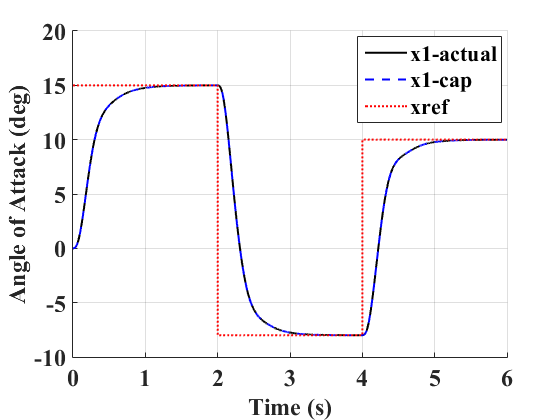
\includegraphics[width=.3\textwidth]{1_ude_varying-mach_x1.png}\hfill
		%	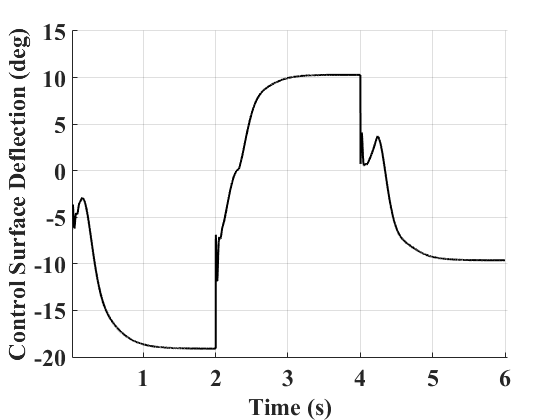
\includegraphics[width=.3\textwidth]{2_ude_varying-mach_control.png}\hfill
		%	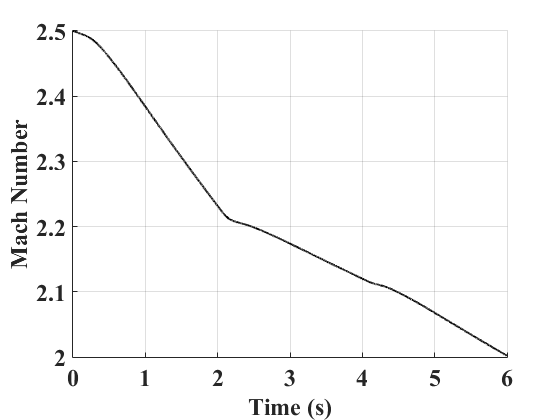
\includegraphics[width=.3\textwidth]{3_ude_varying-mach_mach.png}
		%	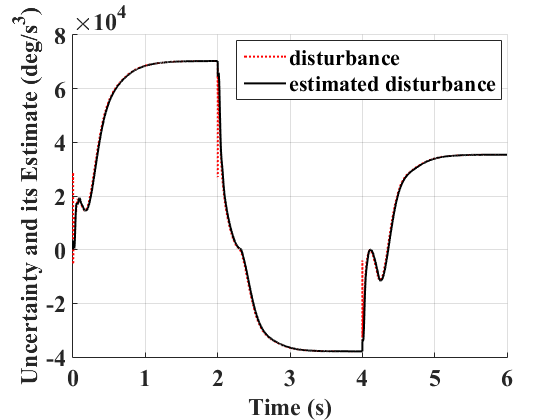
\includegraphics[width=.3\textwidth]{4_ude_varying-mach_dist.png} \hfill
		%	\includegraphics[width=.3\textwidth]{5_ude_varying-mach_obs-err.png} \hfill
		%	\includegraphics[width=.3\textwidth]{6_ude_varying-mach_x1-vs-xcap.png}
		%	%\centerline{\includegraphics[width=.5\textwidth]{5_ude_varying-mach_obs-err.png}}
		%	\caption{Image A.}
		%\end{figure*}
		
	
	\begin{figure*}[h!]
		\centering
		\subfloat[Angle of attack\label{1a}]{%
			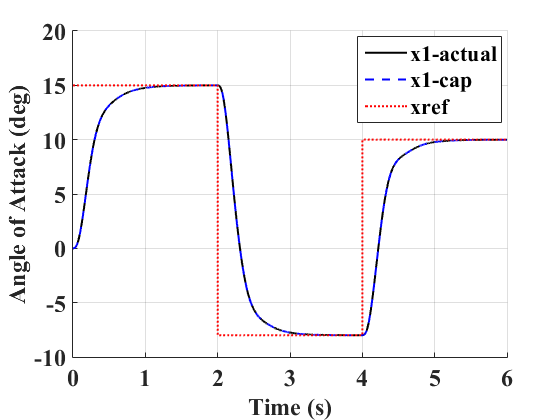
\includegraphics[width=0.3\linewidth]{1_ude_varying-mach_x1.png}}
		\hfill
		\subfloat[Control Effort\label{1b}]{%
			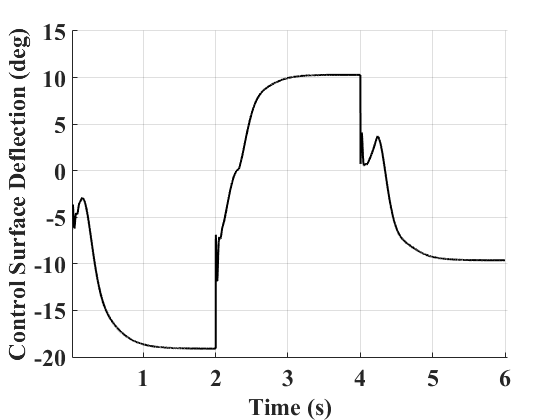
\includegraphics[width=0.3\linewidth]{2_ude_varying-mach_control.png}}
		\hfill
		\subfloat[Mach Dynamics\label{1c}]{%
			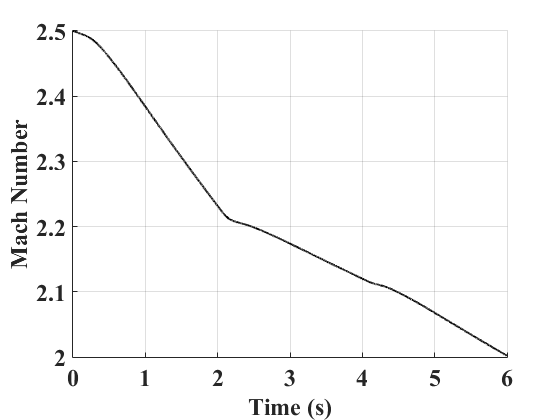
\includegraphics[width=0.3\linewidth]{3_ude_varying-mach_mach.png}}
		\\
		\subfloat[Disturbance Estimation\label{1d}]{% 
			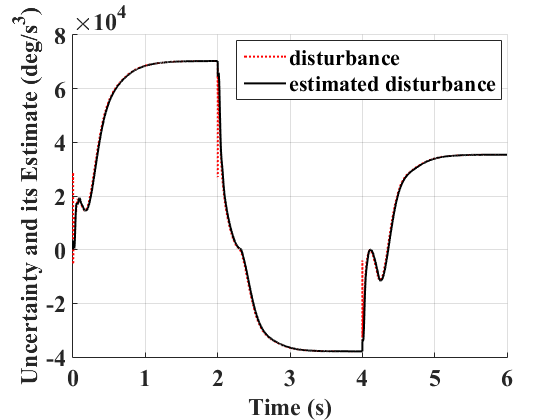
\includegraphics[width=0.3\linewidth]{4_ude_varying-mach_dist.png}}
		%\hfill
		\subfloat[Pitch Rate\label{1e}]{%
			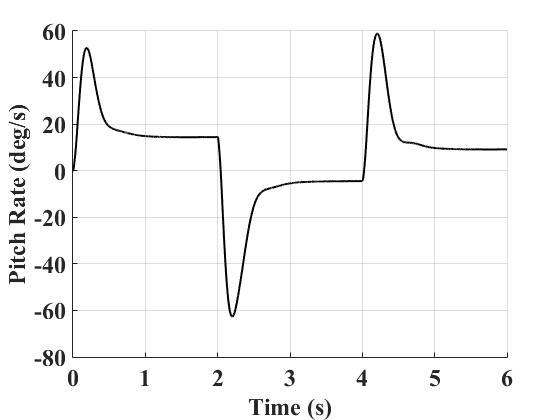
\includegraphics[width=0.3\linewidth]{5_ude_varying-mach_pitch.png}}
		\caption{Performance of UDE augmented IOL controller with Mach dynamics}
		\label{fig1} 
	\end{figure*}
		
	\begin{figure*}[h!]
		\centering
		\subfloat[Angle of attack \label{2a}]{%
			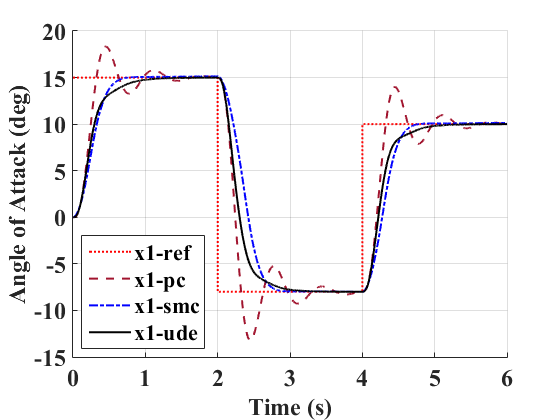
\includegraphics[width=0.3\linewidth]{x1_kcn=1.3_kcm=0.7.png}}
		\hfill
		\subfloat[Pitch \label{2b}]{%
			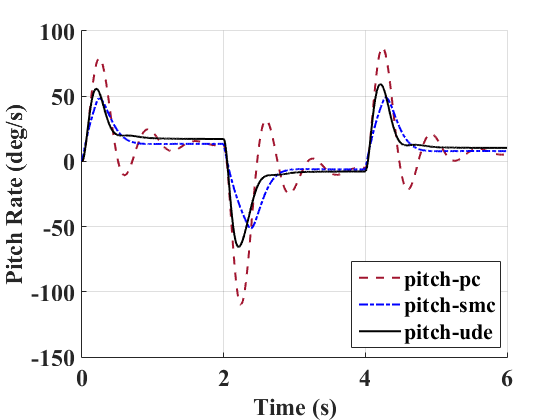
\includegraphics[width=0.3\linewidth]{pitch_kcn=1.3_kcm=0.7.png}}
		\hfill
		\subfloat[Control effort \label{2c}]{%
			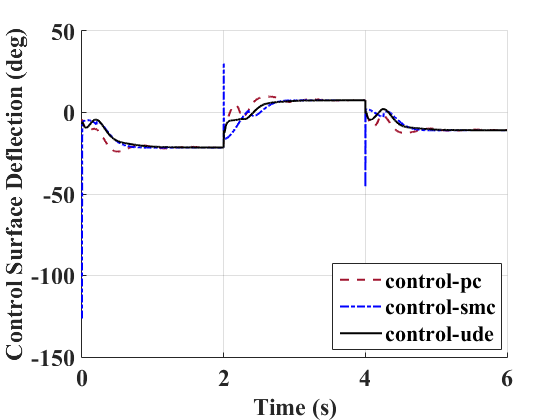
\includegraphics[width=0.3\linewidth]{control_kcn=1.3_kcm=0.7.png}}
		\\	
		\caption{+30\% uncertainty in $C_n$, -30\% uncertainty in $C_m$}
		\label{fig2} 
	\end{figure*}
		
	\subsection*{Case II: Comparative Study With Aerodynamic Uncertainties}
		For comparative analysis of UDE against other control laws, Predictive control (PC) and Sliding mode control (SMC) have been considered. Simulations have been performed by providing an uncertainty of $+30\%$ in aerodynamic force coefficient $C_n$ and $-30\%$ in aerodynamic moment coefficient $C_m$. Mach has been maintained at the nominal constant of $M = 2.25$ and no external disturbances are added to the system.
		\subsubsection{Predictive Control (PC)} 
		This controller has been described in [\ref{pc_talole}] and its adoption to a pitch autopilot has been done in [\ref{eso}]. The following equations describe how PC was implemented for this model;
		\begin{equation}
			u = - \frac{6}{b_p \Delta t^3} \Big[ e + \Delta t\dot{e} + \frac{\Delta t^2}{2}\ddot{e} + \frac{\Delta t^3}{6}(a_p - \dddot{\alpha}^*) \Big] \nonumber
		\end{equation}
		where $\Delta t$ represents the predictive horizon, $e = \alpha - \alpha^*$ is the output tracking error, and the functions $a_p$ and $b_p$ are given as;
		\begin{eqnarray}
			\begin{aligned}
				a_p =& K_qM^2(3a_m\alpha^2+2b_m|\alpha|+c_m\big(-7+\frac{8M}{3})\dot{\alpha} \\ 
				&-K_qM^2d_m\omega_a\delta+K_\alpha M(6a_n\alpha+2b_nsgn(\alpha))\dot{\alpha^2}\\ &+K_\alpha M(3a_n\alpha^2+2b_n|\alpha|+c_n\Big(2-\frac{M}{3}\Big)\ddot{\alpha} \\
				b_p =& K_q M^2d_m\omega_a \nonumber
			\end{aligned}
		\end{eqnarray}		
		In simulations, the value of prediction horizon, $\Delta t = 0.18$ has been used.
		
		\subsubsection{Sliding Mode Control (SMC)}
		SMC has been explored and implemented for a pitch autopilot in [\ref{bahrami}] and the same has been implemented here;
		\begin{eqnarray}
			u = \frac{1}{b_s} ( -\nu(x,t) -\rho sat(s/\phi)) \nonumber
		\end{eqnarray}
		where $s$ is the switching surface given by $s(t) = \dot{e}(t) + \lambda e(t)$ and $e(t) = \alpha - \alpha^*$. $sat(x) = x$ if $|x| \leq 1$, otherwise $sat(x) = sgn(x)$, where $sgn(x)$ itself is equal to $1$ if $x$ is positive, $-1$ if $x$ is negative and zero if $x$ is zero. The quantities $b_s$ and $\nu$ are given as
		\begin{eqnarray}
		\begin{aligned}
		b_s =& K_\alpha M d_n \omega_a	\\
		\nu(x, t) =& \lambda \dot{e} - \ddot{\alpha}^* + K_\alpha M [(3a_n \alpha^2 + 2b_n \mid\alpha\mid \\	
		\quad &+ c_n(2 - M/3)\dot{\alpha} cos(\alpha) - C_n sin(\alpha)\dot{\alpha} )] \\	
		\quad &- K_\alpha M d_n \omega_a \delta + \dot{q} \nonumber
		\end{aligned}
		\end{eqnarray}
		In simulations provided, SMC was used while setting design parameters to $\lambda = 7$, $\rho = 10$, and $\phi = 0.05$ as per [\ref{bahrami}].
		
		\subsection{Comparative Analysis} 
		
		These simulations really help understand and contrast the behavior of the controllers in a situation where uncertainties are present in the system. It can be seen right away from Fig.~(\ref{2a}) and Fig.~(\ref{2b}) that overshoots in PC become much more prominent and even lead to continued oscillations which are not satisfactorily dampened in time. SMC being a robust controller, provides good tracking performance, however, it falters with the control graph Fig.~(\ref{2c}), which contains large spikes in control effort ranging from $\pm 50^\circ$. UDE being the most robust system has smooth tracking, pitch rate and control graphs with no oscillations, settling time as per design and control effort well within the acceptable bounds of $\pm30^\circ$. 
		
		Another point worth noting is that unlike PC and SMC simulations which have used the actual states while implementing the control law, UDE simulation has utilized the estimated states obtained from the UDE observer. As is well known, use of estimated states might result in degraded performance; in contrast the proposed strategy utilizes the estimated states and still proves its worthiness. 
		
		Similar performance was seen for other combinations of uncertainty in $C_n$ and $C_m$.	
				
		%\begin{figure*}[ht!]
		%	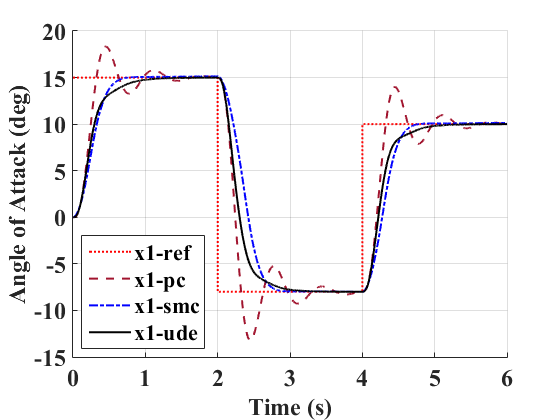
\includegraphics[width=.3\textwidth]{x1_kcn=1.3_kcm=0.7.png}\hfill
		%	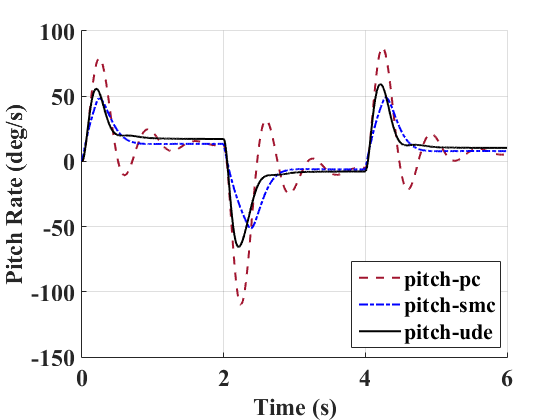
\includegraphics[width=.3\textwidth]{pitch_kcn=1.3_kcm=0.7.png} \hfill
		%	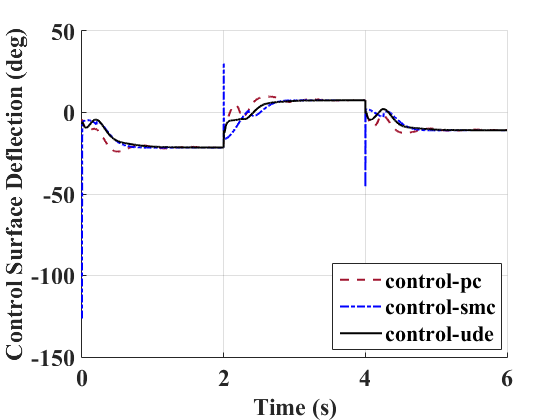
\includegraphics[width=.3\textwidth]{control_kcn=1.3_kcm=0.7.png}
		%	\caption{+30\% uncertainty in Cn, -30\% uncertainty in Cm}
		%\end{figure*}
	
%		\begin{figure*}[h!]
%			\centering
%			\subfloat[Angle of attack \label{2a}]{%
%				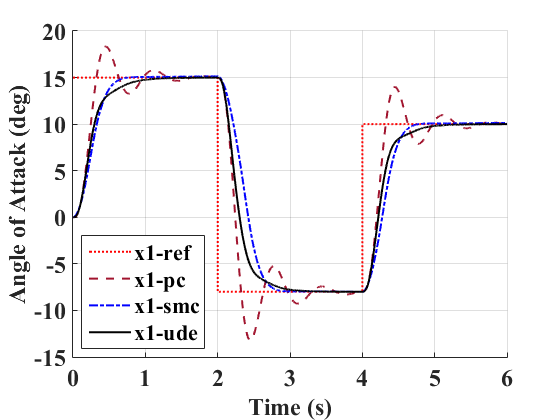
\includegraphics[width=0.3\linewidth]{x1_kcn=1.3_kcm=0.7.png}}
%			\hfill
%			\subfloat[Pitch \label{2b}]{%
%				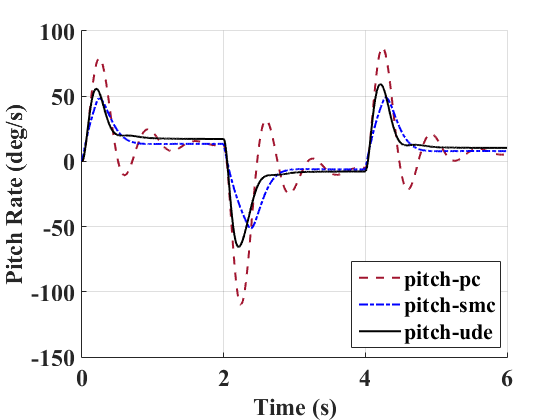
\includegraphics[width=0.3\linewidth]{pitch_kcn=1.3_kcm=0.7.png}}
%			\hfill
%			\subfloat[Control effort \label{2c}]{%
%				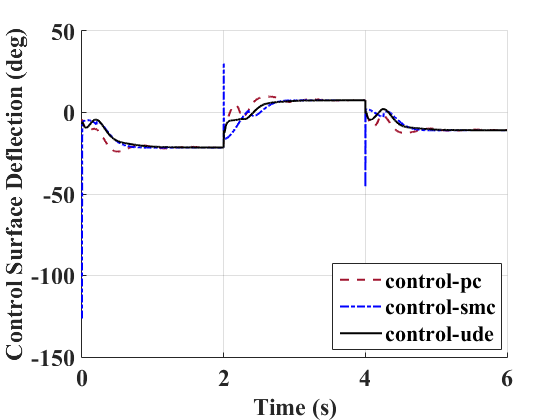
\includegraphics[width=0.3\linewidth]{control_kcn=1.3_kcm=0.7.png}}
%			\\	
%			\caption{+30\% uncertainty in $C_n$, -30\% uncertainty in $C_m$}
%			\label{fig2} 
%		\end{figure*}

\section{Conclusion and Future Work} \label{conclusion}

	In this work, a nonlinear missile model has been considered for the design of a robust pitch autopilot. The dynamics when linearized using IOL was robustified utilizing UDE theory. To address the issue of availability of the states for control law implementation, a UDE based observer has also been designed. Efficacy of the proposed UDE based Controller-Observer structure was tested through numerical simulations and comparative analysis. Simulations have confirmed the robustness property of UDE for this particular aerospace application. 
	
	Our future work would include the design of an integrated pith-yaw-roll autopilot for a nonlinear missile model with and without linearization, using UDE theory.

\begin{thebibliography}{00}
	
	\bibitem{b1} S. H. Kim, Y. S Kim and C. Song, ``A robust adaptive nonlinear control approach to missile autopilot design," Control Eng. Practice, vol. 12, no. 2, pp. 149-–154, 2004. \label{adaptive}
	
	\bibitem{b2} A. R. Mehrabian and J. Roshanian, ``Skid-to-turn missile autopilot design using scheduled eigen structure assignment technique," Proc. Inst. Mech. Eng., Part G: J. Aerosp. Eng., vol. 220, no. 3, pp. 225–-239, 2006. \label{eigen}
	
	\bibitem{b3} S. N. Tiwari, P. N. Dwivedi, A. Bhattacharya and R. Padhi, ``L1 adaptive dynamic inversion missile autopilot with PI structure and adaptive sampling," in 2016 Indian Control Conference (ICC), Hyderabad, pp. 54-59, 2016. \label{L1_adaptive}
	
	\bibitem{b4} Y. Dong, J. Li. and T. Li, ``Generalized extended state observer based H$\infty$ control design for a missile longitudinal autopilot," J. of Aerosp. Eng., vol. 230, no. 12, pp. 2162–-2178, 2015. \label{geso}
	
	\bibitem{b5} S. Bennani, D. M. C Willemsen and C. W. Scherer, ``Robust control of linear parametrically varying systems with bounded rates," J. Guid. Control. Dyn., vol. 21, no. 6, pp. 916--922, 1998. \label{ben}
	
	\bibitem{b6} R. T. Reichert, ``Dynamic scheduling of modern-robust-control autopilot designs for missiles," IEEE Control Systems, vol. 12, no. 5, pp. 35--42, Oct. 1992. \label{rict}
	
	\bibitem{b7} C. Kravaris and M. Soroush, ``Synthesis of multivariable nonlinear controllers by input/output linearization," AIChE J., vol. 36, no. 2, pp. 249-–264, 1990. \label{iol1}
	
	\bibitem{b8} H. R. Karimi and M. R. J. Motlagh, ``Robust Feedback Linearization Control for a non Linearizable MIMO Nonlinear System in the Presence of Model Uncertainties," in 2006 IEEE Int. Conf. on Service Operations and Logistics and Informatics, Shanghai, pp. 965-970, 2006. \label{nonlinear_mimo}
	
	\bibitem{b9} R. Boukezzoula, S. Galichet and L. Foulloy, ``Fuzzy robust control for discrete-time nonlinear systems using input-output linearization and H$\infty$ optimization," in 10th IEEE Int. Conf. on Fuzzy Syst., Melbourne, vol. 3, pp. 765--768, 2001. \label{fuzzy}
	
	\bibitem{b10} J. H. She, S. Hashimoto, T. Yamaura and M. Wu, ``Equivalent-input-disturbance-based high-precision positioning control of dual-stage feed drive," in 2009 Int. Conf. on Netw., Sens., and Control,  Okayama, pp. 398--403, 2009. \label{eid}
	
	\bibitem{b11} S. Li and J. Yang, ``Robust Autopilot Design for Bank-to-Turn Missiles using Disturbance Observers," IEEE Trans. on Aerospace and Electronic Systems, vol. 49, no. 1, pp. 558--579, 2013. \label{dob}
	
	\bibitem{b12} A. A. Godbole, T. R. Libin and S. E. Talole, ``Extended state observer-based robust pitch autopilot design for tactical missiles," J. of Aerosp. Eng., vol. 226, no. 12, pp. 1482–-1501, 2011. \label{eso}
	
	\bibitem{b13}  Q.-C. Zhong and D. Rees, ``Control of uncertain LTI systems based on an uncertainty and disturbance estimator," Journal of Dyn. Sys. Meas. Con.Trans. ASME, vol. 126, no. 4, pp. 905–-910, 2004. \label{ude1}
	
	\bibitem{b14} S.E. Talole, T.S. Chandar and J. P. Kolhe, ``Design and experimental validation of UDE based controller--observer structure for robust input--output linearisation," Int. J. of Control, vol. 84, no. 5, pp. 969-984, 2011. \label{talole2011}
	
	\bibitem{b15} A. Kodhanda, J. Kolhe, T. Zeru and S. Talole, ``Robust aircraft control based on UDE theory", Proc. Inst. Mech. Eng. Part G: J. Aerosp. Eng., vol. 231, no. 4, pp. 728-742, 2017. \label{robust-aircraft-ude}
	
	\bibitem{b16} R. A. Nichols, R. T. Reichert and W. J Rugh, ``Gain scheduling for H-infinity controllers: A flight control example," IEEE Trans. Control Syst. Technol., vol. 1, no. 2, pp. 69–78, 1993. \label{nichols1993}
		
	\bibitem{b17} A. Tsourdos, A. L. Blumel and B. A. White, ``Flight controldesign for amissile-anapproximate feedback linearization approach," in Proc. of the 7th Mediterranean Conf. on Control and Autom. (MED99), Haifa, Israel, pp. 593–602, 1999. \label{rd2}
		
	\bibitem{b18} J. Huang, C. F. Lin, J. R. Cloutier, J. H. Evers and C. D'Souza, "Robust feedback linearization approach to autopilot design," in The First IEEE Conf. on Control Appl., Dayton, pp. 220-225 vol.1., 1992.  \label{huang}	
	
	\bibitem{b19} V. Upreti, S. E. Talole and S. B. Phadke, ``Predictive estimation and control based missile autopilot design," in Proc. AIAA Guid., Navigation, and Control Conf. and Exhibit, Providence, Rhode Island, USA, 2004. \label{pc_talole}
	
	\bibitem{b20} M. Bahrami, B. Ebrahimi, G. R. Ansarifar and J. Roshanian, ``Sliding mode autopilot and observer design for a supersonic flight vehicle," in 2nd Int. Symp. on Syst. and Control in Aerosp. and Astronautics, Shenzhen, pp. 1-5, 2008. \label{bahrami} 
	
	
		
	
\end{thebibliography}


\end{document}
